\section{Introduction}

In EGI era of grid computing in Europe, MyEGEE and Nagios are taking the place
of SAM in performance monitoring of the grid, in NGI oriented infrastructures.
SAM Framework had a significant role in reporting the service availability.
That monitoring model was needed to be replaced by a new Multi Level Monitoring
architecture. The need of establishing a central point in regional level, where
metrics gathered from each information system of the grid, lead to the adoption
of MyOSG. MyEGEE is the tool that extends MyOSG to european NGI's and provides
an interface to customize the display of aggregated metrics of the performance
of NGI sites. Nagios is the main technological choice to provide that regional
monitoring system.

\section{Aims and Objectives}

Different role users are going to use a portal to get information about the
performance status of the grid, to export the appropriate report for their job.
This project aims to develop these particular pieces of code to support the 
aggregation of the metrics from nagios, to allow the web based customization of
the visualization of the reports. These metrics are needed to report the
availability and reliability of NGIs and particular sites of the grid.

The procedures that are going to be used in order to achieve the above aims
should include at the beggining some opening and exploration of the environment
where the interface is going to be placed. The usage of grid computing in
the world should be well known, so a visibility of the importance and the
possible uses of the software will be recognised. The appropriate
access to the infrastructure should be gained, on different platforms and levels.
Brunel University site and GridPP/NGS VO at the beggining, as long as the UKI
ROC operations may be a good point of collaboration with researchers to reach
the bests possible requirements and data to analyse. The middleware used in
both these VOs should be examined so with the knowlege of running projects and
global usage of them may target to export better specifications. Existing
operations on the grid should also be discovered. The european initiative
milestones on the operations of the regional level should be considered as a
route, and registration to news about the upcoming research projects that
are going to use the grid should also be take place.

After that wide-opening to get the whole picture, a targeted and focused
view should follow. Existing monitoring tools must be used to check the problems
and search for requirements. The experience of SAM, Gridview, Gridmap, Gstat,
GridICE, etc should be taken in order to merge their functionality as possible
as it is. Information systems that already reside over the infrastructure, must
also be learned. Standards and specifications should be examined, on how the
message bus works and delivers the data in an hierarhical manner. A contact
with the CERN team working on MyEGEE and Indiana University's MyOSG team should
be established, to collaborate on the core of MyOSG source. Changes submission
to subversion system as long as ticket closure of the development project tool
will help to get to know the core of MyEGEE and Nagios. It is possible to create
and upstream a nagios customized web interface, to create different views of
nagios resources scheme to grid topology oriented architecture. Nagios, NRPE and
Ganglia installations should be deployed across the CE\&SE nodes of Brunel's
sites to have a working production environment to work on. Attention should be
taken on the potential performance impact of these sensors deployment. UKI
MyEGEE validation/testing portal will be used as a pre-production environment
to check changes. PNP should be fixed in GridPP Nagios to be evaluated.
Statistical access log analysis of existing tools may have results on trends of
users/admins prefered views.

Various tools are going to be used to track changes and collaborate. Monitoring
articles in GridPP wiki \& CERN twiki should be made. Snippets upstream \&
status changes must be a regular operation in SVN/JIRA/Trac in CERN interfaces.
Ongoing task through the disseration project is the reading of papers and
methodical updates of Mendeley citation management tool to have the bibliography
organized. Possible changes suggestions to MSc on DCS cource notes about grid
monitoring may by made, as long as the EGI roadmap updates. Finally with the
appropriate supervision and follow-up of meetings and presentations, a paper publishing
might take place.

\section{Literature Review}

Grid computing \cite{li2005grid} is the most recent decade's technology
innovation in high performance computing. A large number of scientistcs working
on the operations of this huge co-operative project of EU. Monitoring \&
information architecture \cite{fisher2002datagrid} has been standardized in the
initial state of that project, to succeed in today scale of 150.000 cores. Use
of grid computing nowadays takes place in academic and research environments,
but applications in industry-based needs such as promising Power Grid control
\cite{Taylor2006} are emerging.

Standards are being published about the operational models that the grid
computing initiative will use. Last decade the EGEE I, II \& III was adopted by
european universities to fund and establish a collaborative community of
researchers under a central point, the CERN oriented research project in
Particle Physics. After EGEE, the European Grid Initiative were formed to lead
to the explode of that community into regional initiatives. Performance
and availability monitoring tools and views also follow that format, phasing out
commonly used SAM \cite{egee3dsa122} and having the adoption of Nagios as the
monitoring of regional performance tool.

Resource Brokers \cite{Kertesz06ataxonomy} where developed to manage the
workload on Computer elements and Resource elements. Globus which is 
non-service based RB was replaced by gLite RB which is service based. A Workload
Management System (WMS) exists in gLite to do the distribution and management of
the Computing and Storage oriented tasks.

A Grid Monitoring Architecture \cite{tierney2002grid} was proposed in early
2000's. Information systems were developed to create repositories of information
needed to be stored for monitoring and statistical reporting reasons. Such an
organized system later was specified by the Aggregated Topology Provider (ATP)
definition. The largest world grids adopt that model, forming OIM in OSG (USA)
and GOCDB as that information base in EGEE (Europe). Message Bus was also
defined as a mean to tranfer the undelying data, and well known tools came up
such as Gstat, GOCDB and BDII with Glue specification. Grid performance
monitoring and keeping of such an information system has also impact in the
performance of the system itshelf \cite{zhang2003performance}, so various
methods were developed to give the solution to the scalling and performance
problem, such as MDS2 (GIIS \& GRIS), GMA and R-GMA
\cite{wilson2004information}, which offers relational environment
\cite{fisher2001relational}, has experience on production systems 
\cite{byrom-production} and scales to reach huge needs such as CMS project
\cite{Bonacorsi2004,Byrom}.

A taxonomy effort has been made \cite{gerndt2004performance} to present the
differencies of performance monitoring systems of the grid, and later a more
general \cite{zanikolas2007importance} taxonomy paper was published to give a
more general visibility of these tools. GridICE was generaly used to aggregate
the performance metrics of ROCs in high level reports
\cite{andreozzi2005gridice}. Later GridICE was left as long as the SAM left, to
meet the milestone of EGI to have a regional monitoring tool (Nagios) to report
the reliability of the joined sites and report the values for SLA reasons.

Latest EGI directive to form regional operation tools pushed the use of Nagios
\cite{imamagic2007grid} as the main tools of availability \& performance (an so
reliability) monitoring of the grid. Each NGI/ROC (regional level) has its own
interface, and hierarhicaly there is a Super Nagios interface to report the top
level view of general system availability. Nagios offers extensions such as NRPE
to remotely invoke check commands in inaccesible/private installations.
Another important add-on to Nagios is the NdoUtils, which offers an SQL store
of history data to the monitoring interface. Nagios Configuration Generator was
introduced to help the automaticaly generation of the configuration based on
the information system of nodes and services. Finally, there has been proposed
an integration of SAM views to a Nagios customized interface, to offer the last
good known SAM interface to the old users. Nagios also integrates with GGUS, a
ticketing system that european grid initiative uses.

Brunel Univesity takes part in regional and european initiatives. 4 different
Computer Elements exist, and 3 Storage Elements, consisting the UKI-LT2-Brunel
site. LT2 stands for London Grid, a co-operation with other London Universities.
GridPP and NGS are two collaboration groups that Brunel Univesity is member of,
and papers on the web interface \cite{Hobson2007} and real time visualization of
the grid status were presented \cite{Huang2007} by GridPP.

\section[Experimental]{Experimental/investigative methods to be adopted}

To develop the interface of customized views of aggregated performance metrics,
an initial evaluation of the underlying information systems must be made. Data
repositories and technologies that specifies the message bus, such as LDAP/BDII,
SQL/R-GMA, XML multicast/Ganglia and file logging/ndo2db-SQL of Nagios should be
evaluated. 

The views that are needed, based on the appropriate roles (users,
operators/admins, managers) must be specified before deciding which hierarhical
model view will be choosen. There should be checked whether it is useful to
layer the views to service/node/site/NGI/VO reports or to target to a specific.

The language that is going to be used to aggregate the underlying data should
also be chosen at this point. MyEGEE is PHP  based, Nagios core is based in
opensource CGI and plugins are bash/perl scripts. Nagios web interface plugins
are usually in PHP/Python. The integration of Nagios and BDII using NCG should
take care of exit status of Nagios commands, that should be interpreted
numerical values of services/resources metrics. It is possible to create custom
nagios plugins-check scripts. 

The decision of how special graphs are going to be
created should be also made. Using standard libraries such as rrdtool, or
whether to aggregate the already generated by the new Gstat 2.0 graphs.
There are also two ways of generation of the graphs. Generation of graphs may be
followed by disk caching using files, or on demand generation using a php/python
script throughing binary image headers to produce graphs. Mixed environment is
another solution to exceed speed due to caching of common used graphs, and
flexibility in rare reports. There should also be decided if Ganglia
gmond/gmetad metrics are going to be aggregated in the MyEGEE. 

Finally, security
using authentication should be checked in the whole tree of the portal, and
performance tuning queries should be always be an ongoing task to reach the
required scalling of use of the interface.

\begin{table}[ht]
\begin{tabular}{ | l | l | l | l | r |}    
\hline
Task & Start date & End date & Duration in days \\ \hline
  Preliminary & 03/29/10 & 04/24/10 & 20 \\ \hline 
  -  Identify Concepts & 03/29/10 & 04/08/10 & 8 \\ \hline 
  -  Gain Access & 04/08/10 & 04/24/10 & 12 \\ \hline 
  Planning & 05/12/10 & 06/04/10 & 17 \\ \hline 
  -  Explore existing technologies & 05/12/10 & 05/28/10 & 12 \\ \hline 
  -  Write Interim Report & 05/28/10 & 06/04/10 & 5 \\ \hline 
  Experimental-Development & 06/04/10 & 08/14/10 & 51 \\ \hline 
  -  Evaluate performance monitoring tools & 06/04/10 & 06/25/10 & 15 \\ \hline 
  -  Information/topology databases & 06/17/10 & 06/29/10 & 8 \\ \hline 
  -  Develop Customized Interface & 06/29/10 & 08/14/10 & 34 \\ \hline 
  ---    Coding of information aggregation & 06/29/10 & 07/21/10 & 16 \\ \hline 
  ---    Development of the frontend & 07/21/10 & 08/10/10 & 14 \\ \hline 
  ---    Complete the interface (auth, scale, etc) & 08/10/10 & 08/14/10 & 4 \\
      \hline Report & 08/16/10 & 09/29/10 & 32 \\ \hline 
  -  Begin Writing & 08/17/10 & 09/01/10 & 11 \\ \hline 
  -  Submit Draft \& Make Changes & 09/01/10 & 09/14/10 & 9 \\ \hline 
  -  Prepare Final & 09/14/10 & 09/29/10 & 11 \\ \hline 
\end{tabular}
%\caption{Key activities necessary to complete the project}
\label{tab:tasks}
\end{table}


\section[Time plan]{Time-plan (Gantt Chart)}

\tikzstyle{line} = [draw]

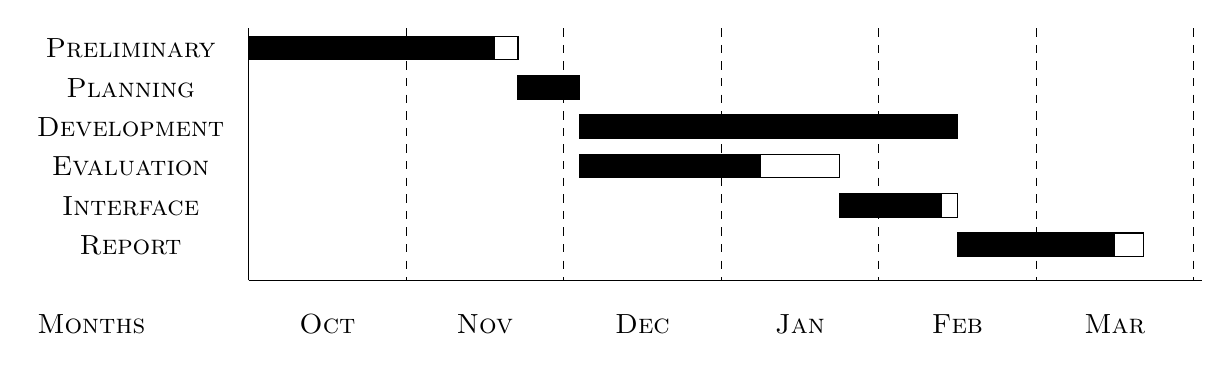
\begin{tikzpicture}
%\draw[help lines] (0,0) grid +(10,1);
%lines
\draw (0,0) -- (0,-3.2);
%\path [line,dashed] (1,0) -- (1,-5.7);
\path [line,dashed] (2,0) -- (2,-3.2);
%\path [line,dashed] (3,0) -- (3,-5.7);
\path [line,dashed] (4,0) -- (4,-3.2);
%\path [line,dashed] (5,0) -- (5,-5.7);
\path [line,dashed] (6,0) -- (6,-3.2);
%\path [line,dashed] (7,0) -- (7,-5.7);
\path [line,dashed] (8,0) -- (8,-3.2);
%\path [line,dashed] (9,0) -- (9,-5.7);
\path [line,dashed] (10,0) -- (10,-3.2);
%\path [line,dashed] (11,0) -- (11,-5.7);
\path [line,dashed] (12,0) -- (12,-3.2);

\draw (-1.5,-0.5) node[above]{$ \textsc{Preliminary}$};%
\draw (-1.5,-1) node[above]{$ \textsc{Planning}$};%
\draw (-1.5,-1.5) node[above]{$ \textsc{Development}$};%
\draw (-1.5,-2) node[above]{$ \textsc{Evaluation}$};%
\draw (-1.5,-2.5) node[above]{$ \textsc{Interface}$};%
\draw (-1.5,-3) node[above]{$ \textsc{Report}$};%
%\draw (-1.5,-3.5) node[above]{$ \textsc{activity G}$};%
%\draw (-1.5,-4) node[above]{$ \textsc{activity H}$};%
%\draw (-1.5,-4.5) node[above]{$ \textsc{activity I}$};%
%\draw (-1.5,-5) node[above]{$ \textsc{activity J}$};%
%\draw (-1.5,-5.5) node[above]{$ \textsc{Report}$};%

\filldraw[fill=white] (0,-0.1) rectangle (3.42,-0.4);% a slack
\filldraw[fill=black] (0,-0.1) rectangle (3.12,-0.4);% a
\filldraw[fill=white] (3.42,-0.6) rectangle (4.2,-0.9);% b slack
\filldraw[fill=black] (3.42,-0.6) rectangle (4.2,-0.9);% b
\filldraw[fill=black] (4.2,-1.1) rectangle (9,-1.4);% c
\filldraw[fill=white] (4.2,-1.6) rectangle (7.5,-1.9);% d slack
\filldraw[fill=black] (4.2,-1.6) rectangle (6.5,-1.9);% d
\filldraw[fill=white] (7.5,-2.1) rectangle (9,-2.4);% e slack
\filldraw[fill=black] (7.5,-2.1) rectangle (8.8,-2.4);% e
\filldraw[fill=white] (9,-2.6) rectangle (11.36,-2.9);% k slack
\filldraw[fill=black] (9,-2.6) rectangle (11,-2.9);% k
%\filldraw[fill=white] (3.2,-2.6) rectangle (6.66,-2.9);% f slack
%\filldraw[fill=black] (3.2,-2.6) rectangle (3.4,-2.9);% f
%\filldraw[fill=white] (7,-3.1) rectangle (9.6,-3.4);% g slack
%\filldraw[fill=black] (7,-3.1) rectangle (8,-3.4);% g
%\filldraw[fill=white] (7,-3.6) rectangle (7.53,-3.9);% h slack
%\filldraw[fill=black] (7,-3.6) rectangle (7.43,-3.9);% h 
%\filldraw[fill=black] (6.66,-4.1) rectangle (7.53,-4.4);% i 
%\filldraw[fill=black] (7.53,-4.6) rectangle (9.58,-4.9);% i 

\draw (0,-3.2) -- (12,-3.2);
\draw (0,-3.2) -- (12.1,-3.2);


\draw (-2,-4) node[above]{$ \textsc{Months}$};%
\draw (1,-4) node[above]{$ \textsc{Oct}$};%
%\draw (1,-6.5) node[above]{$ \textsc{21}$};%
\draw (3,-4) node[above]{$ \textsc{Nov}$};%
%\draw (3,-6.5) node[above]{$ \textsc{23}$};%
\draw (5,-4) node[above]{$ \textsc{Dec}$};%
%\draw (5,-6.5) node[above]{$ \textsc{25}$};%
\draw (7,-4) node[above]{$ \textsc{Jan}$};%
%\draw (7,-6.5) node[above]{$ \textsc{27}$};%
\draw (9,-4) node[above]{$ \textsc{Feb}$};%
%\draw (9,-6.5) node[above]{$ \textsc{29}$};%
\draw (11,-4) node[above]{$ \textsc{Mar}$};%
%\draw (11,-6.5) node[above]{$ \textsc{31}$};%
%\draw (12,-6.5) node[above]{$ \textsc{}$};%
\end{tikzpicture}



\pagebreak
\section[Deliverables]{Deliverables or specific outcomes}

\begin{itemize}
  \item Standards based monitoring environment for the UKI-LT2-Brunel site
  \item Site level Nagios web interface with PNP vizualization graphs for the
  report of Nagios check commands, NRPE installations if needed for the
  different CEs/SEs for the UKI-LT2-Brunel
  \item Site level Ganglia monitoring. Gmond \& Gmetad installations in every
  node of every CE/SE of UKI-LT2-Brunel
  \item Region level customized MyEGEE, to offer basic customization of taken
  metrics. The aggregation should be made based on the previous SAM views. That
  MyEGEE will be installed in validation/testing UKI MyEGEE.
  \item Region level Nagios web interface, with PNP vizualization graphs for the
  report of member-sites availability based on the taken metric at a higher
  level.
  \item A number of submissions to the MyOSG/MyEGEE project at Indiana
  University and CERN repositories.
\end{itemize}